\begin{figure}[h!]
  \centering
\tikzset{every picture/.style={line width=0.75pt}} %set default line width to 0.75pt

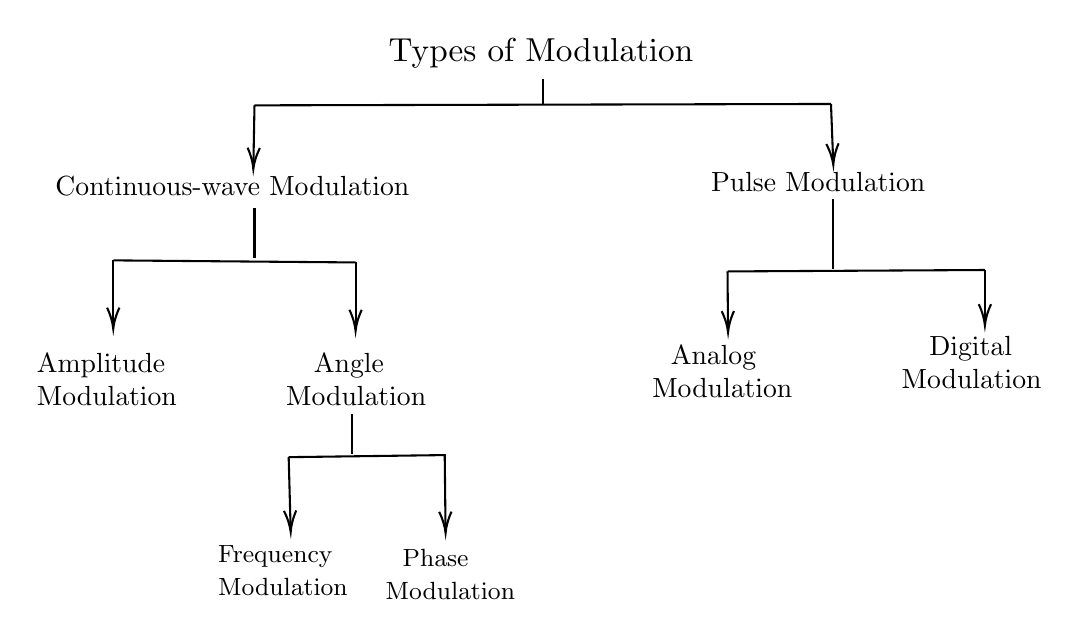
\begin{tikzpicture}[x=0.7pt,y=0.75pt,yscale=-1,xscale=0.9]
%uncomment if require: \path (0,473.3333282470703); %set diagram left start at 0, and has height of 473.3333282470703

\draw    (228.67,146.67) -- (228.67,177.67) ;
\draw [shift={(228.67,179.67)}, rotate = 270] [color={rgb, 255:red, 0; green, 0; blue, 0 }  ][line width=0.75]    (10.93,-3.29) .. controls (6.95,-1.4) and (3.31,-0.3) .. (0,0) .. controls (3.31,0.3) and (6.95,1.4) .. (10.93,3.29)   ;

\draw    (89.67,145.67) -- (89.67,176.67) ;
\draw [shift={(89.67,178.67)}, rotate = 270] [color={rgb, 255:red, 0; green, 0; blue, 0 }  ][line width=0.75]    (10.93,-3.29) .. controls (6.95,-1.4) and (3.31,-0.3) .. (0,0) .. controls (3.31,0.3) and (6.95,1.4) .. (10.93,3.29)   ;

\draw    (89.67,145.67) -- (228.67,146.67) ;


\draw    (170.67,120.67) -- (170.67,144.67) ;


\draw    (190.29,240.48) -- (279.79,239.48) -- (280.26,274.98) ;
\draw [shift={(280.29,276.98)}, rotate = 269.24] [color={rgb, 255:red, 0; green, 0; blue, 0 }  ][line width=0.75]    (10.93,-3.29) .. controls (6.95,-1.4) and (3.31,-0.3) .. (0,0) .. controls (3.31,0.3) and (6.95,1.4) .. (10.93,3.29)   ;

\draw    (190.29,240.48) -- (191.39,274.47) ;
\draw [shift={(191.45,276.47)}, rotate = 268.15999999999997] [color={rgb, 255:red, 0; green, 0; blue, 0 }  ][line width=0.75]    (10.93,-3.29) .. controls (6.95,-1.4) and (3.31,-0.3) .. (0,0) .. controls (3.31,0.3) and (6.95,1.4) .. (10.93,3.29)   ;

\draw    (226.56,219.46) -- (226.56,238.79) ;


\draw    (442,151) -- (589.63,150.31) ;


\draw    (442,151) -- (442.28,178.31) ;
\draw [shift={(442.3,180.31)}, rotate = 269.40999999999997] [color={rgb, 255:red, 0; green, 0; blue, 0 }  ][line width=0.75]    (10.93,-3.29) .. controls (6.95,-1.4) and (3.31,-0.3) .. (0,0) .. controls (3.31,0.3) and (6.95,1.4) .. (10.93,3.29)   ;

\draw    (589.63,150.31) -- (589.63,174.98) ;
\draw [shift={(589.63,176.98)}, rotate = 270] [color={rgb, 255:red, 0; green, 0; blue, 0 }  ][line width=0.75]    (10.93,-3.29) .. controls (6.95,-1.4) and (3.31,-0.3) .. (0,0) .. controls (3.31,0.3) and (6.95,1.4) .. (10.93,3.29)   ;

\draw    (502.68,116.31) -- (502.68,149.64) ;


\draw    (170.68,70.98) -- (501.34,70.31) ;


\draw    (336.01,58.31) -- (336.01,70.64) ;


\draw    (170.68,70.98) -- (170.05,99.64) ;
\draw [shift={(170.01,101.64)}, rotate = 271.25] [color={rgb, 255:red, 0; green, 0; blue, 0 }  ][line width=0.75]    (10.93,-3.29) .. controls (6.95,-1.4) and (3.31,-0.3) .. (0,0) .. controls (3.31,0.3) and (6.95,1.4) .. (10.93,3.29)   ;

\draw    (501.34,70.31) -- (502.59,97.65) ;
\draw [shift={(502.68,99.64)}, rotate = 267.4] [color={rgb, 255:red, 0; green, 0; blue, 0 }  ][line width=0.75]    (10.93,-3.29) .. controls (6.95,-1.4) and (3.31,-0.3) .. (0,0) .. controls (3.31,0.3) and (6.95,1.4) .. (10.93,3.29)   ;


\draw (335,46) node [scale=1.2,color={rgb, 255:red, 0; green, 0; blue, 0 }  ,opacity=1 ] [align=left] {Types of Modulation};
\draw (158,110) node  [align=left] {Continuous-wave Modulation};
\draw (494,108) node  [align=left] {Pulse Modulation};
\draw (86,203) node  [align=left] {Amplitude \\Modulation};
\draw (229,203) node  [align=left] { \ \ \ Angle\\Modulation};
\draw (187,295) node  [align=left] {{\small Frequency}\\{\small Modulation}};
\draw (283,297) node  [align=left] {{\small  \ \ Phase}\\{\small Modulation}};
\draw (439,199) node  [align=left] { \ \ Analog\\Modulation};
\draw (582,195) node  [align=left] { \ \ \ Digital\\Modulation};


\end{tikzpicture}
\label{fig:f1}
\caption{Types of Modulation}
\end{figure}
